% Preamble
\documentclass[11pt]{article}

    % Packages
    \usepackage{a4wide}
    \usepackage[utf8]{inputenc}
    \usepackage[T1]{fontenc}
    \usepackage[naustrian]{babel}
    
    \usepackage{verbatim}
    \usepackage{enumerate}
    \usepackage{scrextend}
    \usepackage{graphicx}
    
    \title{Rechnerorganisation - 2. Klausurvorbereitung}
    \author{Auer Thomas}
    \date{\today}

\begin{document}
\maketitle
\tableofcontents
\graphicspath{{graphics/}}
\pagebreak
\section{Übungsblatt 5}
    \subsection{Multi-Cycle Datenpfad: lw-Instruktion}
    \textbf{Erläutern Sie die Ausführung der lw-Instruktion (load word) für den Multi-Cycle-Datenpfad.
    Welche Vorteile bietet der Multi-Cycle-Datenpfad gegenüber dem Single-Cycle-Datenpfad?
    Diskutieren Sie dies anhand dieses Befehls.}

    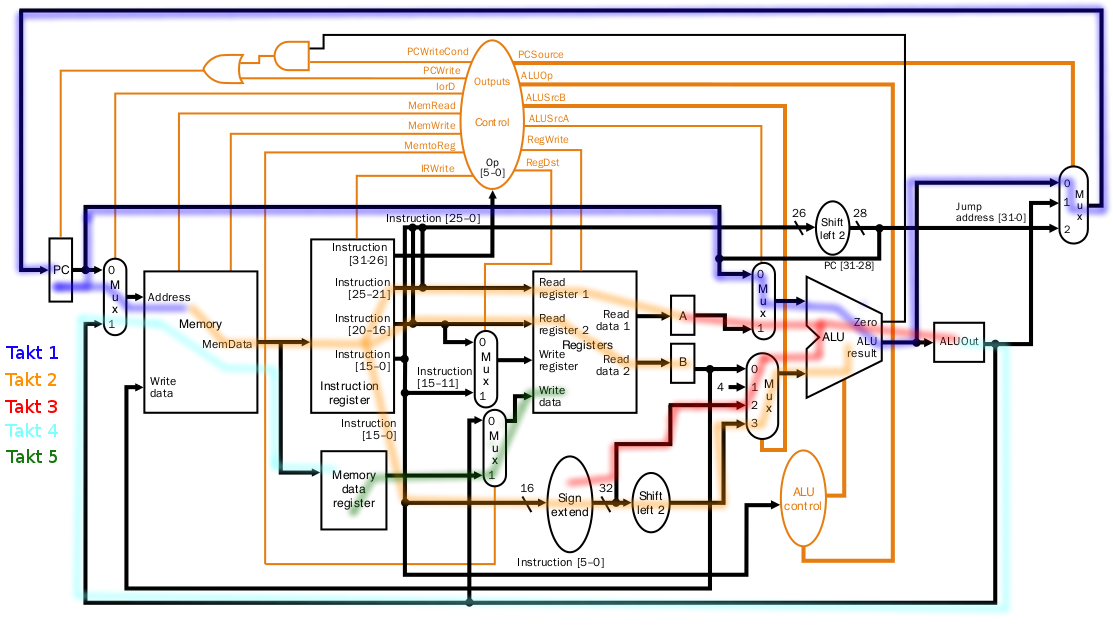
\includegraphics[width=\textwidth]{LW_MCDp}

    \subsection{Grundlagen Pipelining}
    \textbf{Gegeben seien vier unterschiedliche Prozessoren, die sich in der Anzahl der Pipelinestufen und
    der Taktrate unterscheiden:\\}
    \begin{center}
        \begin{tabular}{l|l|l}
        Prozessor & Pipelinestufen & Taktrate \\\hline
        A & 1 & 100 MHz \\
        B & 4 & 800 MHz \\
        C & 12 & 1,5 GHz \\
        D & 20 & 3,2 GHz \\
        \end{tabular}
    \end{center}
    \textbf{(a) Bestimmen Sie für jeden Prozessor die Latenz der einzelnen Instruktionen.}
    
    \textbf{Wie lange dauert die Ausführung von 400.000 voneinander unabhängigen Instruktionen
    auf jedem der angeführten Prozessoren? Bestimmen Sie die Performance und den
    Speedup verglichen mit Prozessor A ohne Pipelining. (Sie können annehmen, dass es
    keine Stalls gibt.)}

    \subsection{Pipelining: Graphische Darstellung}

    \textbf{Beantworten Sie folgende Fragen anhand der Beispiel-Pipeline-Architektur der VO (Kapitel 3.2).\\\\
    (a) Bestimmen Sie die Anzahl der Pipelinestufen, die Taktdauer und die Taktfrequenz der
    Beispiel-Pipeline unter Annahme der Angaben auf VO-Folie 3-44 (Ausführungszeiten der
    Funktionseinheiten). Wie lange dauert die Ausführung eines einzigen Befehls auf der
    Beispiel-Pipeline?\\\\
    (b) Angenommen es treten keine Leertakte (stalls) auf, welchen Speedup erreicht die
    Beispiel-Pipeline aus a) gegenüber einem Single-Cycle Datenpfad, der aus den gleichen
    Funktionsregistern besteht?\\
    Seite 1 von 2\\\\
    (c) Auf der Pipeline wird folgende Befehlssequenz ausgeführt:\\}
    \begin{verbatim}
        and     $10, $2, $3
        sw      $11, 4($3)
    \end{verbatim}

    \textbf{    Stellen Sie die Ausführung der oben angeführten Befehlssequenz durch die Beispiel-Pipeline
    wie auf VO-Folie 3-45 grafisch dar (untere Abbildung). Achten Sie insbesondere auf die
    zeitliche Anordnung der Zugriffe auf die Registereinheit! Wie lange dauert die Ausführung der
    Befehlssequenz?}


    \subsection{Pipelining: Daten- und Kontrollabhängigkeiten}
    \textbf{Gegeben sei folgendes Code-Fragment:}

    \begin{center}
        
    \includegraphics[width=0.5\textwidth]{5_4}
    
    \end{center}

    \textbf{(a) Identifizieren Sie alle Daten- und Kontrollabhängigkeiten, die Leerzyklen (Stalls)
    verursachen (Annahme: ohne Forwarding-Einheit). Wie viele Taktzyklen werden für die
    Ausführung des gesamten Codes bzw. pro Ergebniselement (d.h. nur die Schleife)
    benötigt?\\\\
    (b) Welche aus den Datenabhängigkeiten resultierenden Pipeline-Konflikte können durch
    eine Forwarding-Einheit gelöst werden? Wie viele Taktzyklen benötigt die Ausführung der
    Befehlssequenz mit Forwarding-Einheit für die Ausführung des gesamten Codes bzw. pro
    Ergebniselement (d.h. nur die Schleife)? Wo und warum muss die Hardware Leerzyklen
    (d.h. Stalls) einfügen?\\\\
    (c) Ordnen Sie den Code so um, dass er auf einer modifizierten Beispiel-Pipeline mit
    Unterstützung für „Delayed Branching“ (d.h. Branch-Delay-Slot) möglichst rasch
    ausgeführt wird (und die Semantik erhalten bleibt). Wie viele Taktzyklen werden in diesem
    Fall für die Ausführung des gesamten Codes bzw. pro Ergebniselement (d.h. nur die
    Schleife) benötigt? Wie hoch ist der erzielte Speedup relativ zu bzw. b)?}


\section{Übungsblatt 6}


\section{Übungsblatt 7}


\section{Übungsblatt 8}


\section{Übungsblatt 9}


\section{Übungsblatt 10}

    
\end{document}